% Experiment 2, restyled from the user's Elegant_Project_Report_Template.tex.
% Content: Qi's reviewed V3 report and this experiment's archived evidence only.
% Compile from this directory: tectonic QYY_Experiment_2_Report.tex
\documentclass[11pt,a4paper]{article}

\usepackage[T1]{fontenc}
\usepackage{newtxtext,newtxmath}
\usepackage[scaled=0.92]{helvet}
\usepackage[scaled=0.88]{inconsolata}
\usepackage[table]{xcolor}
\usepackage[left=22mm,right=22mm,top=23mm,bottom=22mm]{geometry}
\usepackage{graphicx,booktabs,tabularx,float,caption,enumitem,listings}
\usepackage{fancyhdr,titlesec,lastpage,microtype,hyperref}
% Explicit OpenType bindings prevent TU/phv and TU/zi4 fallback under Tectonic.
% TeX Gyre Heros preserves the template's Helvetica-style sans serif.
\usepackage{fontspec}
\setsansfont{texgyreheros-regular.otf}[BoldFont=texgyreheros-bold.otf,
  ItalicFont=texgyreheros-italic.otf,BoldItalicFont=texgyreheros-bolditalic.otf,Scale=.92]
\setmonofont{Inconsolatazi4-Regular.otf}[BoldFont=Inconsolatazi4-Bold.otf,
  Scale=.88,Mapping=,Ligatures=NoCommon]
\usepackage{amsmath,tikz,pgfplots}
\usetikzlibrary{arrows.meta,positioning}
\pgfplotsset{compat=1.18}
\graphicspath{{assets/}}
\newcolumntype{Y}{>{\raggedright\arraybackslash}X}
\setlength{\parindent}{0pt}
\setlength{\parskip}{5pt}
\setlength{\emergencystretch}{2em}
\renewcommand{\arraystretch}{1.18}

% ---------- Personal information and project fields ----------
\newcommand{\ReportTitle}{Fixed-Point Grasping\\with RoboMaster EP}
\newcommand{\ReportSubtitle}{Experiment 2\\Records and Result Analysis}
\newcommand{\ReportCourse}{Robotics Integration Group Project I}
\newcommand{\ReportShortTitle}{Experiment 2 / RoboMaster EP}
\newcommand{\ReportAuthor}{Yongyue Qi}
\newcommand{\ReportRepository}{\href{https://github.com/ccx8kg5qpd-debug/robomaster-ep-fixed-point-grasping}{GitHub / shared project}}
\newcommand{\ReportDate}{13 September 2026}
\newcommand{\ReportKeywords}{Fixed-point grasping / Simulation / Evidence analysis}
\newcommand{\StudentID}{24020036050}

% ---------- Colour system ----------
\definecolor{Ink}{HTML}{102A43}
\definecolor{Blue}{HTML}{1261A0}
\definecolor{Teal}{HTML}{168C8C}
\definecolor{Sky}{HTML}{DDEFF7}
\definecolor{Mist}{HTML}{F2F6F8}
\definecolor{Gold}{HTML}{E5A13A}
\definecolor{Text}{HTML}{253746}
\definecolor{Muted}{HTML}{647685}
\definecolor{Card}{HTML}{173F5F}

\hypersetup{colorlinks=true,linkcolor=Blue,urlcolor=Teal,citecolor=Teal,
  pdftitle={Fixed-Point Grasping with RoboMaster EP},pdfauthor={\ReportAuthor},
  pdfsubject={Experiment 2: records and result analysis},
  pdfkeywords={RoboMaster EP, fixed-point grasping, simulation, evidence analysis}}

\pagestyle{fancy}
\fancyhf{}
\setlength{\headheight}{15pt}
\fancyhead[L]{\sffamily\small\color{Muted}\ReportShortTitle}
\fancyhead[R]{\sffamily\small\color{Muted}\ReportAuthor}
\fancyfoot[L]{\sffamily\scriptsize\color{Muted}\ReportKeywords}
\fancyfoot[R]{\sffamily\scriptsize\color{Muted}Page \thepage\ of \pageref{LastPage}}
\renewcommand{\headrulewidth}{0.4pt}

\titleformat{\section}{\sffamily\Large\bfseries\color{Ink}}
  {\colorbox{Teal}{\textcolor{white}{\thesection}}}{0.7em}{}
\titleformat{\subsection}{\sffamily\large\bfseries\color{Blue}}
  {\thesubsection}{0.6em}{}
\titlespacing*{\section}{0pt}{16pt}{8pt}
\titlespacing*{\subsection}{0pt}{12pt}{5pt}
\setlist[itemize]{leftmargin=1.6em,itemsep=2pt,topsep=4pt}
\captionsetup{font=small,labelfont={bf,sf,color=Ink},textfont={color=Muted}}

\lstset{basicstyle=\ttfamily\small,backgroundcolor=\color{Mist},frame=single,
  rulecolor=\color{Sky},breaklines=true,columns=fullflexible,showstringspaces=false,upquote=true,
  xleftmargin=0.4em,xrightmargin=0.4em,aboveskip=7pt,belowskip=7pt}

\newcommand{\metriccard}[2]{\colorbox{Card}{\parbox[c][24mm][c]{0.43\textwidth}{
  \centering\sffamily\textcolor{Sky}{\small\MakeUppercase{#1}}\\[2pt]
  \textcolor{white}{\Large\bfseries #2}}}}
\newcommand{\callout}[1]{\begin{center}\fcolorbox{Teal}{Mist}{
  \parbox{0.91\textwidth}{\color{Text}\small #1}}\end{center}}
\newcommand{\code}[1]{{\small\nolinkurl{#1}}}
\newcommand{\source}[1]{{\small\color{Muted}Source: #1}\par}
\tikzset{record/.style={draw=Teal,fill=Mist,rounded corners=2pt,
  align=center,font=\small,minimum height=12mm,text width=43mm},
  link/.style={-{Latex[length=2mm]},thick,draw=Teal}}

\begin{document}
\hypersetup{pageanchor=false}
\begin{titlepage}
\pagecolor{Ink}\color{white}\thispagestyle{empty}
\vspace*{18mm}
{\sffamily\small\bfseries\color{Gold}\MakeUppercase{\ReportCourse}\par}
\vspace{8mm}
{\sffamily\fontsize{30}{36}\selectfont\bfseries\ReportTitle\par}
\vspace{3mm}
{\sffamily\fontsize{22}{28}\selectfont\color{Sky}\ReportSubtitle\par}
\vspace{10mm}{\color{Teal}\rule{\textwidth}{2.2pt}}\vspace{12mm}

\noindent
\metriccard{Main simulation}{5 / 5 cycles}\hfill
\metriccard{Mean simulation error}{4.358 mm}\\[6mm]
\metriccard{Max. simulation error}{5.604 mm}\hfill
\metriccard{Hardware: team-observed}{5 / 5 transfers}

\vfill
\renewcommand{\arraystretch}{1.55}
\noindent\begin{tabularx}{\textwidth}{>{\sffamily\bfseries\color{Sky}}l X}
Author & \textbf{\ReportAuthor} \\
Student ID & \StudentID \\
Repository & \ReportRepository \\
Report date & \ReportDate \\
Document & English individual laboratory report \\
\end{tabularx}
\vspace{8mm}{\color{Gold}\rule{\textwidth}{1.2pt}}
\end{titlepage}

\hypersetup{pageanchor=true}
\nopagecolor\color{Text}
\renewcommand{\arraystretch}{1.18}
\setcounter{tocdepth}{1}
\tableofcontents
\vspace{12mm}
\callout{\textbf{Reading the results.} The millimetre values on the cover come from
the main simulation record. The hardware outcome is the team's confirmation of
five successful transfers with no observed abnormalities; it is not a measurement
of physical placement precision.}
\vspace{5mm}
{\small\color{Muted}This individual report focuses on experiment records and
result analysis. Its content is based on the reviewed Experiment 2 report and
the matching project archive. The QYY personal template supplies the visual
design only. Body page numbering starts with this contents page; the cover is
unnumbered.}
\clearpage

\section{Experiment Requirements and Individual Scope}
\label{sec:scope}
\subsection{Task and platform adaptation}
The task is fixed-point grasping without visual localization: home, approach A,
descend, grip, lift, transfer to B, release and return. The course handout requires
a complete simulation launch, state publication, saved trajectories/results/errors,
joint and reachability checks, and at least four successful transfers in five
consecutive trials. Hardware work additionally requires supervised low-speed
operation, safe failure handling and individual safety-operation checks [1].

Because of equipment availability, our group used the DJI RoboMaster EP arm and
gripper instead of the specified mechArm 270. The simulation uses ROS 2 Humble,
Gazebo Fortress and custom kinematics/control on a Jetson Linux system. The
physical implementation uses the RoboMaster Python SDK. This is a platform
adaptation, not an unchanged ROS 2 hardware backend.

\subsection{My responsibility and the team's interfaces}
My main responsibility is organizing simulation results and report material.
I use the files supplied by the simulation members to summarize the five trials,
calculate placement errors and explain the results. The hardware pair provides
the physical-test outcome. My role does not include operating the real robot or
claiming authorship of the simulation code.

\begin{table}[H]
\centering\small
\caption{Shared division of work and my reporting scope}
\begin{tabularx}{\textwidth}{@{}p{27mm}p{27mm}Y@{}}
\toprule
Member & Work area & Main responsibility\\\midrule
Ning Bo & Simulation & Environment and scene setup; model loading and launch.\\
Huang Junbiao & Simulation & Motion programming; grasp, transfer and repeated-cycle debugging.\\
Yongyue Qi & Simulation results & Log organization, numerical analysis and report material.\\
Xue Yutong & Hardware & Pick/release waypoints, approach/lift heights, gripper adjustment and retention checks; joint trials.\\
Bao Lintai & Hardware & SDK communication, task sequence, chassis turn/return and exceptions; joint trials.\\
\bottomrule
\end{tabularx}
\end{table}
The two hardware members share physical setup, parameter review and integrated
five-cycle testing. Their technical focuses differ, but neither is assigned a
permanent passive-helper role. Each student remains responsible for the analysis
in their own individual report.

\callout{\textbf{Scope of evidence.} Simulation repeats A$\rightarrow$B and verifies
home after every cycle, with object replenishment between cycles. Hardware
alternates A/B, pauses for human grasp confirmation and returns home after all
five cycles. The shared-interface/parameter-only migration objective and each
member's safety-operation check are not demonstrated by the supplied records.}
\clearpage

\section{Principles of a Verifiable Grasping Experiment}
\label{sec:principles}
\subsection{From motion to acceptance evidence}
The simulation sequence is home, hover, descend, close, hold, lift, turn, lower,
open and retreat. Placement verification is followed by heading restoration and
arm homing. Only then is a successful cycle appended to the results. A box
reaching B alone does not prove completion of the full cycle, including return.

The scene contains a 25 mm cube and fixed world points
$A=(0.278,-0.001,0.0725)$ m and $B=(0.237,0.1453,0.0725)$ m. Fresh bilateral
contact feedback triggers a small closure preload. HOLD has a nominal 3 s
duration, followed by verification conditions that must remain satisfied for
at least 0.4 s before lifting. Transfer uses chassis rotation plus small position
corrections; the arm is not treated as a six-axis industrial manipulator.

\begin{figure}[H]
\centering
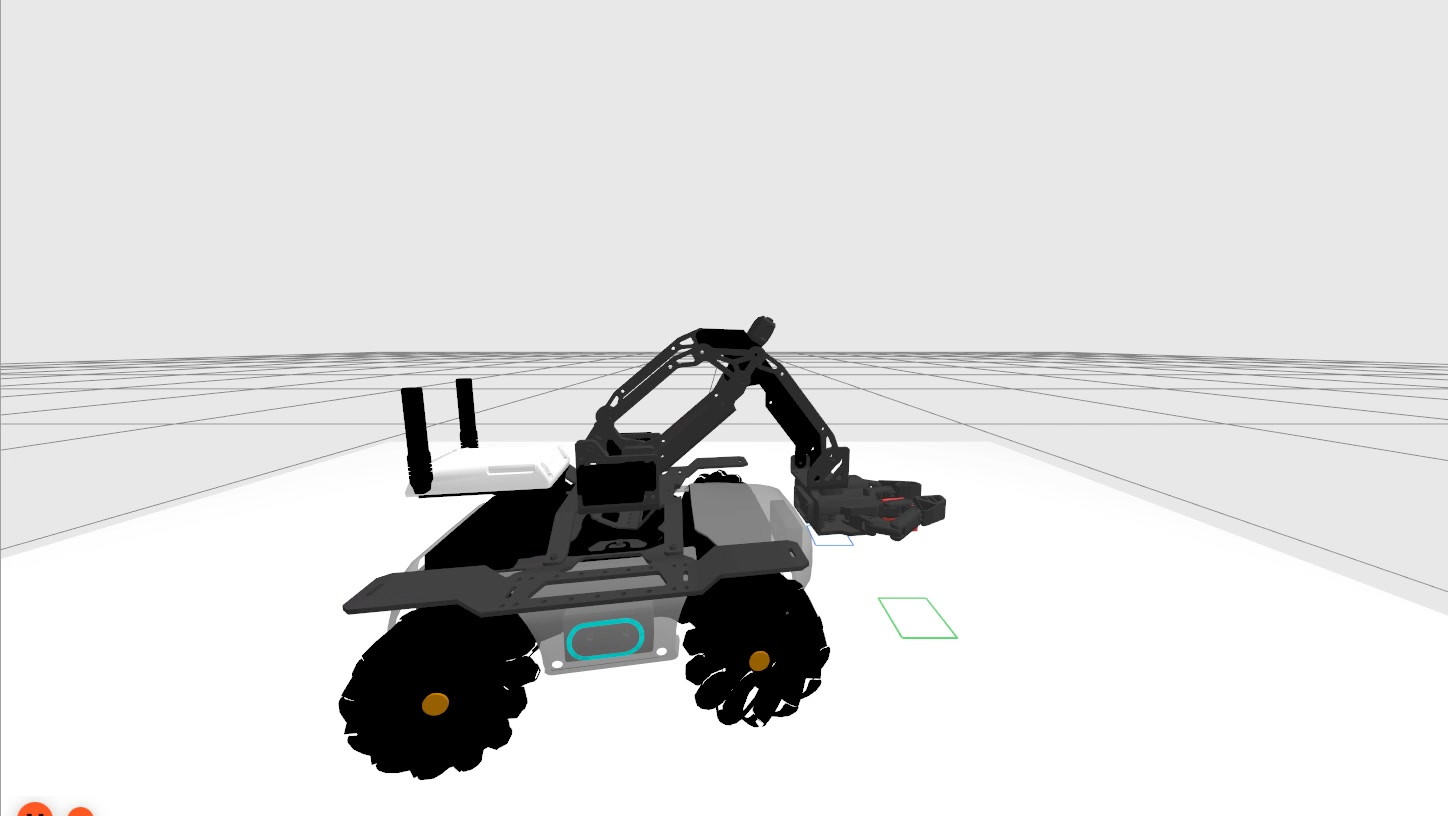
\includegraphics[width=.92\textwidth,trim=0 20 0 210,clip]{simulation_lift.jpg}
\caption{Scene frame from the team's Experiment 2 simulation recording at 34 s.
This is a simulation view, not a photograph of the hardware or an error measurement.}
\label{fig:scene}
\end{figure}

\subsection{Definitions and units}
For recorded placement $(x_i,y_i,z_i)$ and target $(x_B,y_B,z_B)$ in metres,
the horizontal placement error is
\begin{equation}
e_{xy,i}=1000\sqrt{(x_i-x_B)^2+(y_i-y_B)^2}\quad\mathrm{mm},
\qquad \bar e=\frac{1}{5}\sum_{i=1}^{5}e_{xy,i}.
\label{eq:error}
\end{equation}
The controller's configured acceptance test requires $e_{xy}<23$ mm,
$|z_i-z_B|<8$ mm and recent table contact. These are program thresholds, not
millimetre tolerances specified by the course handout. The sample mean is not
a guaranteed accuracy specification. Heading error is the absolute difference
from the initial chassis heading at the home check.

Cycle duration uses a monotonic wall clock and includes execution and waiting
under the actual computer load. The first cycle includes initial homing; later
cycles start after refill. The first cycle's additional time should not be
interpreted as degradation in grasping performance.
\clearpage

\section{Record Audit and Reproducibility}
\label{sec:audit}
\subsection{Selecting one authoritative run}
The main quantitative record is the recording-associated run
\code{20260913_153855_682865}. The earlier run
\code{20260913_151835_077998} remains a separate comparison. Both completed five
simulation cycles, but their coordinates and timestamps must not be merged.
The main run's saved configuration has \code{autostart=false}, consistent with
manual task initiation for filming; the earlier run uses \code{autostart=true}.

\begin{figure}[H]
\centering
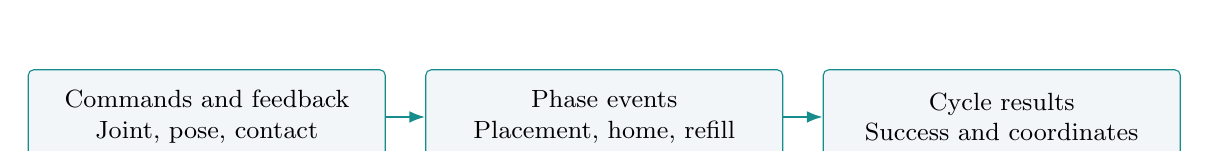
\begin{tikzpicture}[node distance=5mm]
\node[record] (s) {Commands and feedback\\Joint, pose, contact};
\node[record,right=of s] (e) {Phase events\\Placement, home, refill};
\node[record,right=of e] (r) {Cycle results\\Success and coordinates};
\draw[link] (s)--(e);\draw[link] (e)--(r);
\end{tikzpicture}
\caption{Complementary records used to check a completed simulation cycle.}
\end{figure}

\begin{table}[H]
\centering\small
\caption{Evidence inventory for the main simulation run}
\begin{tabularx}{\textwidth}{@{}p{33mm}Yp{25mm}@{}}
\toprule
Evidence & What it establishes & Count\\\midrule
\code{results.json} & Requested/completed cycles; placement and home outcomes. & 5 / 5 cycles\\
\code{events.jsonl} & Phase transitions and verification order. & 81 events\\
Placement events & Box accepted at B. & 5\\
Home events & Return verified before success is recorded. & 5\\
Refill request / ack & Replenishment between completed cycles. & 4 / 4\\
\code{trajectory.csv} & Sampled robot/object feedback, including idle time. & 4,475 rows\\
\bottomrule
\end{tabularx}
\end{table}

\subsection{Checking order and elapsed time}
The event log contains 60 phase entries, one run-start event and one completion
event. No \code{SAFE_STOP} event appears. This supports normal completion, not
successful testing of the stop branch. Four refill operations are expected:
the fifth cycle ends the task instead of preparing a sixth object.

Initial-home entry to run completion spans approximately 318.02 s. The five
saved cycle durations sum to 310.03 s; approximately 7.99 s lies outside those
intervals, including refill-related transitions. The 329.13 s video contains
recording time outside active execution. The trajectory also includes idle
time, so its full span is not the task duration.

\subsection{Keeping the evidence chain intact}
I use result coordinates for numerical errors, events for ordering, and
trajectory data for feedback history. Video supplies scene context but cannot
independently establish millimetre-level placement. Analysis should retain the
original B coordinate, compute at full precision, and round only displayed values.
Each success must match placement and home checks, and each refill must follow
home verification. An abandoned script's failure is development history, not a
failure of the final five-cycle hardware run confirmed by the team.
\clearpage

\section{Simulation Results and Error Interpretation}
\label{sec:results}
\begin{table}[H]
\centering
\caption{Five-cycle main-run results, with home verified after every transfer}
\begin{tabular}{@{}crrrcc@{}}
\toprule
Cycle & Error (mm) & Heading ($^\circ$) & Time (s) & Placed & Home\\\midrule
1 & 2.274 & 0.445 & 67.01 & Yes & Yes\\
2 & 5.604 & 0.329 & 59.72 & Yes & Yes\\
3 & 4.192 & 0.404 & 60.92 & Yes & Yes\\
4 & 4.577 & 0.459 & 61.09 & Yes & Yes\\
5 & 5.144 & 0.405 & 61.29 & Yes & Yes\\
\bottomrule
\end{tabular}
\end{table}
\source{Main-run \code{results.json}. Error is horizontal distance from B;
heading is absolute home-heading error; time is the saved cycle wall duration.}

\begin{figure}[H]
\centering
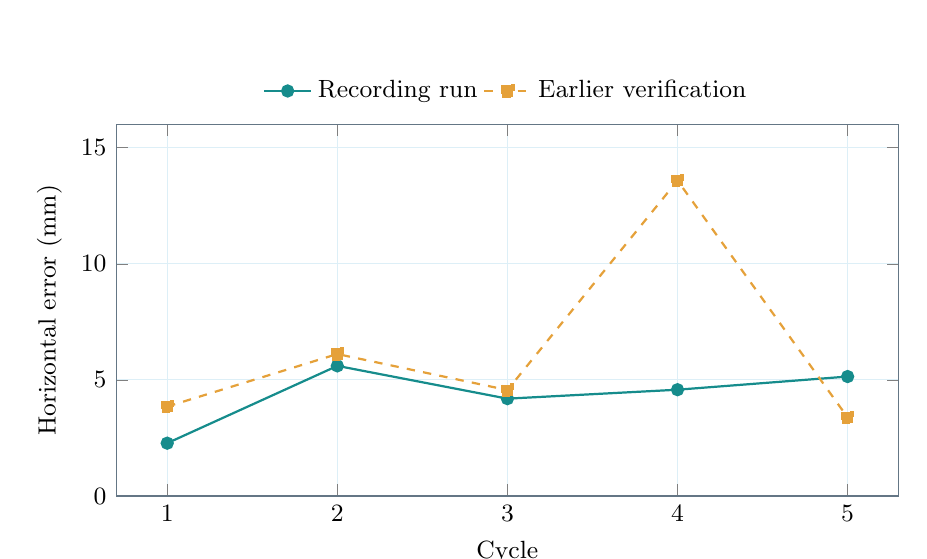
\begin{tikzpicture}
\begin{axis}[width=.95\textwidth,height=63mm,ymin=0,ymax=16,xmin=.7,xmax=5.3,
xtick={1,2,3,4,5},xlabel={Cycle},ylabel={Horizontal error (mm)},grid=major,
grid style={draw=Sky},legend style={font=\small,draw=none,at={(.5,1.03)},
anchor=south,legend columns=2},tick label style={font=\small},
label style={font=\small},axis line style={draw=Muted}]
\addplot+[color=Teal,mark=*,mark options={draw=Teal,fill=Teal},thick] coordinates
{(1,2.273879)(2,5.603849)(3,4.191550)(4,4.577359)(5,5.143734)};
\addlegendentry{Recording run}
\addplot+[color=Gold,mark=square*,mark options={draw=Gold,fill=Gold},dashed,thick] coordinates
{(1,3.849790)(2,6.113820)(3,4.561980)(4,13.585014)(5,3.382556)};
\addlegendentry{Earlier verification}
\end{axis}
\end{tikzpicture}
\caption{Two distinct five-cycle simulation runs. Neither series is hardware data.}
\label{fig:errors}
\end{figure}

\callout{\textbf{Main-run result:} 5/5 accepted placements and five verified
returns home. Mean horizontal error is 4.358 mm; maximum error is 5.604 mm.
Both are below the controller's configured 23 mm horizontal threshold.}

The earlier run's mean was 6.299 mm, with a 13.585 mm fourth-cycle error. That
larger value remains a successful placement under the same positional threshold
and must not be omitted. The lower mean in the recording run does not prove a
controlled algorithmic improvement: these are two small runs, not a randomized
comparison with repeated conditions. The defensible conclusion is successful
execution in both datasets with visible run-to-run variability.

The saved home arm error of about $4.21\times10^{-14}$ rad reflects idealized
numerical feedback, not physical positioning precision. I report this as a
passed home condition rather than an advertised accuracy figure.
\clearpage

\section{Hardware Outcome and Simulation Differences}
\label{sec:hardware}
\subsection{Team-observed physical validation}
The team confirmed that the hardware trials took place on 12 September 2026,
with five successful transfers and no observed abnormalities using the final
manual-confirmation workflow. Each lift was
followed by a fresh human \code{y} confirmation before rotation; heading
restoration and arm homing followed cycle 5. This is an observed 5/5 result,
not an instrumented precision or timing measurement.

\begin{table}[H]
\centering
\caption{Hardware outcomes confirmed by the team, not an automatic test log}
\begin{tabular}{@{}clll@{}}
\toprule
Cycle & Direction & Outcome & Abnormality\\\midrule
1 & A$\rightarrow$B & Successful & None observed\\
2 & B$\rightarrow$A & Successful & None observed\\
3 & A$\rightarrow$B & Successful & None observed\\
4 & B$\rightarrow$A & Successful & None observed\\
5 & A$\rightarrow$B & Successful & None observed\\
\bottomrule
\end{tabular}
\end{table}

\subsection{Why the implementations must not be conflated}
The archived hardware program uses the RoboMaster SDK, lifts from
\code{GRASP=(191,-51)} to \code{HOVER=(191,-1)} in SDK millimetres, stops the
chassis and waits up to 30 s for confirmation. The 50 mm difference is a
commanded lift, not an independently measured object displacement. Odd cycles
turn $+32^\circ$ and even cycles $-32^\circ$. No confirmation means no transfer
turn or automatic return; cleanup attempts to pause the gripper, stop the base
and close the SDK connection. This is not a certified emergency-stop circuit.

\begin{table}[H]
\centering\small
\caption{Differences retained in the analysis}
\begin{tabularx}{\textwidth}{@{}p{27mm}YY@{}}
\toprule
Aspect & Final simulation & Final hardware\\\midrule
Control route & ROS 2, bridge and Gazebo controllers & Direct RoboMaster SDK\\
Direction & A$\rightarrow$B each cycle & Alternating A/B\\
Grasp decision & Bilateral contact and object height & Human confirmation after lift\\
Return & Home verified every cycle & Initial home and final return after cycle 5\\
Replenishment & Four resets after home verification & No automatic cube refill\\
Evidence & Coordinates, events and trajectory & Team-observed successes\\
\bottomrule
\end{tabularx}
\end{table}

\callout{\textbf{Do not transfer simulation precision to hardware.} No measured
physical placement errors, forces, durations or object mass were supplied.
The model's 50 g cube mass is not a real weighing. Five successful transfers
meet the observed success-count criterion for this sample, but do not establish
long-run reliability or complete compliance with every course requirement.}
\clearpage

\section{Problems, Solutions and Individual Reflection}
\label{sec:reflection}
\subsection{Version ambiguity and inconsistent claims}
The development history includes object-animation experiments and an abandoned
hardware checking script. Mixing these versions could produce contradictory
claims about automatic object detection and manual confirmation. I anchor final
behavior in the archived code and use conversation notes for development history.
Simulation, final hardware outcomes and historical tests remain separate.

\subsection{Success flags without sufficient context}
A success flag is meaningful only when its conditions are understood. Here,
placement checks horizontal distance, height and table contact; home verification
follows separately. My solution is to cross-check coordinates against the target
and join the result with the placement/home events, rather than treat either a
closed gripper or a visually plausible video as sufficient evidence.

\subsection{Offline tests versus system-level fault evidence}
The fact-check record reports four passing offline tests on the final simulation
code. One calls \code{Kinematics().solve(10,10,0.6)} and expects
\code{ValueError} for an unreachable target. This establishes solver-level
rejection, not the running system's stopping response. No complete final-version
system-level fault-injection campaign is documented. Further tests should cover
runtime target rejection, stale pose feedback, failed grasping and blocked refill,
recording the expected error, observed state and stopping behavior separately.

\subsection{A fair account of the adapted experiment}
The recorded simulation and team-observed hardware both meet the success-count
criterion. Direct SDK control and hardware end-only return nevertheless differ
from the handout's shared-interface and parameter-only-switching objectives.
The evidence also does not document each member's individual safety-operation
check. I acknowledge these boundaries instead of equating 5/5 transfers with
complete compliance.

\subsection{Conclusion and next improvement}
My contribution is an auditable account of the experiment, not a claim of
personally programming or operating every subsystem. Experimental quality depends
on traceable definitions as much as on a successful demonstration. A useful next
step would attach a common trial identifier to video, telemetry and result files,
then collect real placement measurements with a consistent reference. This would
support a defensible simulation-to-hardware comparison without inventing precision.

\callout{\textbf{Conclusion.} The final records support five successful simulated
cycles with per-cycle home verification and five team-confirmed physical
transfers without observed abnormalities. Numerical precision is established
only for the saved simulation sample; unrecorded tests remain unverified.}
\clearpage

\section{Shared GitHub Repository and Commit Evidence}
\label{sec:repository}
The complete group archive is stored in the
\href{https://github.com/ccx8kg5qpd-debug/robomaster-ep-fixed-point-grasping}
{shared private GitHub repository}. The repository address is
\nolinkurl{github.com/ccx8kg5qpd-debug/robomaster-ep-fixed-point-grasping}.
It contains the
simulation and hardware programs, model resources, saved results, the complete
simulation recording and all five individual report sources. The real-hardware
video remains explicitly marked as pending and will be added after recording.

\begin{figure}[H]
\centering
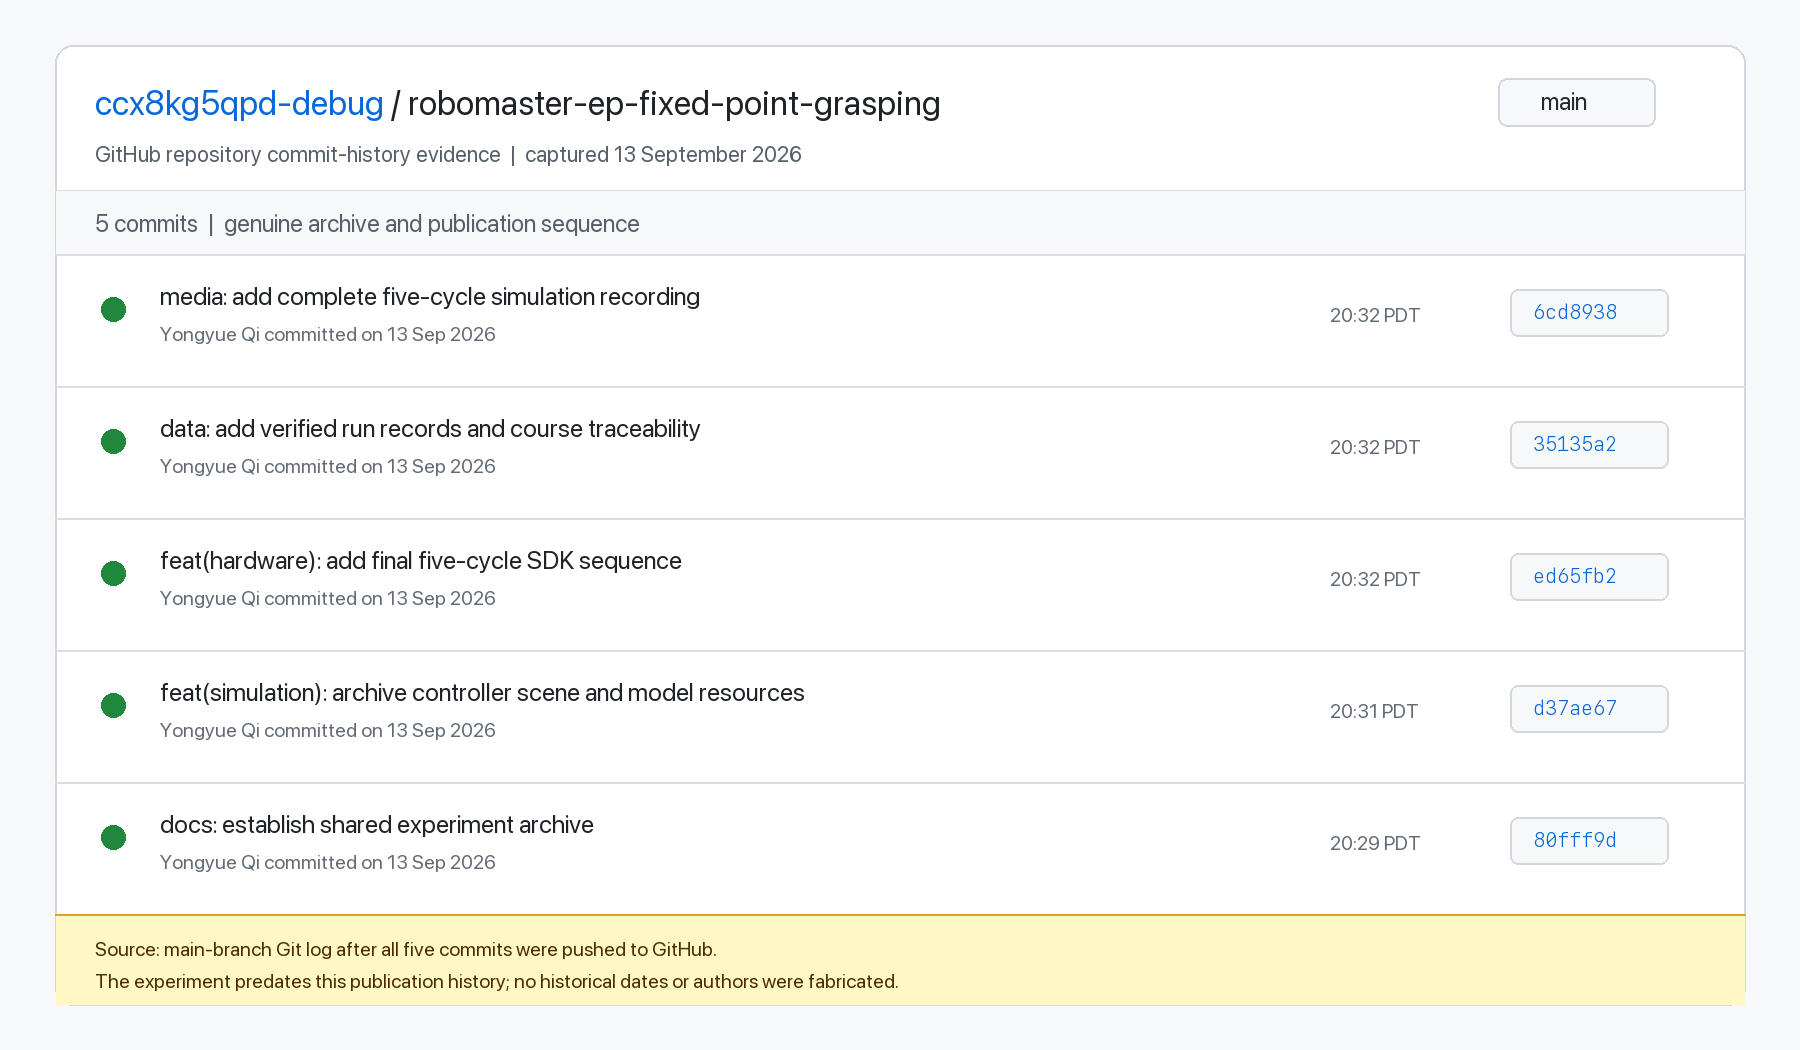
\includegraphics[width=\linewidth]{commit_history_snapshot.png}
\caption{Commit-history evidence captured after the first five project-material
commits had been pushed to the shared GitHub repository.}
\end{figure}

\callout{\textbf{Traceability note.} The experiment was completed before the
GitHub repository was assembled. These genuine commits document the later review,
organization and publication sequence; they are not presented as a fabricated
contemporaneous development history. The image records the five commits visible
at capture time, before this revised report was added.}
\clearpage

\section{Sources, Reproduction and Evidence Limits}
\label{sec:sources}
\subsection{Sources and traceability}
{\small
[1] Current course handout, \emph{Robotics Integration Group Project I:
Fixed-Point Robotic-Arm Grasping, Simulation Development and Hardware
Validation}, S16--S20 / E5, and the individual-report assignment requirements.
The course field is translated from this experiment's handout.\par
[2] Shared team repository,
\href{https://github.com/ccx8kg5qpd-debug/robomaster-ep-fixed-point-grasping}
{robomaster-ep-fixed-point-grasping}, assembled 13 September 2026:
simulation source/configuration, \code{real_v2_five_cycles_manual.py}, saved
results, event log and trajectory. Main run: \code{20260913_153855_682865};
comparison run: \code{20260913_151835_077998}.\par
[3] Team conversation fact-check materials dated 13 September 2026 for
development and offline-test history; subsequent team confirmation for the
successful final five-cycle hardware run.\par
[4] Community model resources: \href{https://github.com/jeguzzi/robomaster_ros}
{jeguzzi/robomaster\_ros}, archived commit \code{c05a39d7f0fa}.
This dependency repository is not the team's experiment repository.\par
[5] Author's QYY personal layout, \code{Elegant_Project_Report_Template.tex}.
Earlier QYY work was consulted for visual design only. No previous experiment's
body, images, metrics or conclusions were reused.\par
}

\subsection{Reproducing the numerical summary}
Unmodified copies of both result files, the main event log and its trajectory
are included in \code{supporting_data/}. The packaged \code{check_numbers.py}
recomputes errors, cycle totals and event counts without starting a simulator
or connecting to a robot. The analysis below illustrates the same calculation;
it is report-analysis code, not the robot controller.

\begin{lstlisting}[language=Python,caption={Horizontal-error calculation from the saved main-run record}]
import json, math, statistics
from pathlib import Path
run = "20260913_153855_682865"
path = Path("supporting_data") / run / "results.json"
data = json.loads(path.read_text())
bx, by, _ = data["configuration"]["b_world_m"]
errors_mm = []
for cycle in data["cycles"]:
    x, y, _ = cycle["placement_world_m"]
    errors_mm.append(1000 * math.hypot(x - bx, y - by))
print(statistics.mean(errors_mm), max(errors_mm))
\end{lstlisting}

\subsection{Record availability and experimental limitations}
\begin{itemize}
\item \textbf{Repository:} the group uses the shared private repository linked
in Section~\ref{sec:repository}. Its publication commits were made after the
experiment and are described as archive history, not experimental-development
history. No previous-project repository is substituted.
\item \textbf{Dates:} the team-confirmed hardware trial date is 12 September 2026.
The cover date, 13 September 2026, is the report-preparation date.
\item \textbf{Evidence limits:} no additional physical placement, timing, force
or mass measurements, individual safety-check records or system-level fault-test
records were supplied. These properties are not inferred from the team-observed
5/5 outcome. The offline-test evidence described in Section~\ref{sec:reflection}
remains distinct from unrecorded system-level tests.
\end{itemize}

\end{document}
